\documentclass[11pt,twocolumn]{article}

%%%%%%%%%%%%%%%%%%%%%%%%%%%%%%%%%%%%%%%%%%%%%%%%%%%%%%%%%%%%%%%%%%%%%%%%%%%%%%%%%%
\usepackage{url}
\usepackage[breaklinks]{hyperref}
\usepackage{breakurl}

\usepackage{graphicx}

\usepackage[svgnames]{xcolor} 

\usepackage{amsmath}
\usepackage{amsfonts}
\usepackage{amssymb}

\usepackage[top=2.5cm, bottom=2.5cm, left=2.5cm, right=2.5cm]{geometry}

\usepackage{comment}

%%%%%%%%%%%%%%%%%%%%%%%%%%%%%%%%%%%%%%%%%%%%%%%%%%%%%%%%%%%%%%%%%%%%%%%%%%%%%%%%%%
\usepackage{natbib}
\bibliographystyle{unsrtnat}

\renewcommand*{\bibfont}{\footnotesize}

%%%%%%%%%%%%%%%%%%%%%%%%%%%%%%%%%%%%%%%%%%%%%%%%%%%%%%%%%%%%%%%%%%%%%%%%%%%%%%%%%%

\usepackage{ntheorem}
\makeatletter
\renewtheoremstyle{plain}% Adds automatic line break, if heading is too long
  {\item{\theorem@headerfont ##1\ ##2\theorem@separator}~}
  {\item{\theorem@headerfont ##1\ ##2\ (##3)\theorem@separator}~}
\makeatother

\newtheorem{theorem}{Theorem}%[section]
\newtheorem{mydef}{Definition}[section]
\newtheorem{corollary}{Corollary}[section]




%%%%%%%%%%%%%%%%%%%%%%%%%%%%%%%%%%%%%%%%%%%%%%%%%%%%%%%%%%%%%%%%%%%%%%%%%%%%%%%%%%
% correct bad hyphenation here
\hyphenation{op-tical net-works semi-conduc-tor}

%%%%%%%%%%%%%%%%%%%%%%%%%%%%%%%%%%%%%%%%%%%%%%%%%%%%%%%%%%%%%%%%%%%%%%%%%%%%%%%%%%
% 
\newcommand{\DERPAR}[4]{\frac{\partial #1_{#3}(\mathbf{\hat{#2}})}{ \partial \hat{#2}_{#4}}}

%%%%%%%%%%%%%%%%%%%%%%%%%%%%%%%%%%%%%%%%%%%%%%%%%%%%%%%%%%%%%%%%%%%%%%%%%%%%%%%%%%
% paper title
\title{An Optimal Method for Tuning a Six-Hole Ocarina }

\author{Fernando Pujaico Rivera}

\date{ }

\begin{document}



% keywords: Resonator, Whistles, Helmholtz, ocarina
% make the title area
\maketitle


\begin{abstract}
In this paper we propose an optimal method for tuning a six-hole ocarina,
this optimization will be subordinated by the minimization of 
the square norm of square difference between the desired and obtained resonant frequency.
The results show that it is not possible to tune a John Taylor style six-hole ocarina with a perfect equal temperament scale, 
but the minimization rule returns a tuning method with an optimal approximation and heterogeneous errors less than $35.613\%$ of a semitone.
\end{abstract}



%%%%%%%%%%%%%%%%%%%%%%%%%%%%%%%%%%%%%%%%%%%%%%%%%%%%%%%%%%%%%%%%%%%%%%%%%%%%%%%%
%%%%%%%%%%%%%%%%%%%%%%%%%%%%%%%%%%%%%%%%%%%%%%%%%%%%%%%%%%%%%%%%%%%%%%%%%%%%%%%%
\section{Introduction}
The ocarina is an extremely ancient musical instrument widely used in worldwide. 
It is classified as a globular flute and
depending on the culture we can find shapes like animals, vegetables or anthropomorphic.
Exist vestiges of clay ocarinas in 
Shang dynasty peoples in Bronze Age China, 
Bantu peoples of Southern Africa,
pre-Columbian cultures in Peru, etc.
\citep[pp. 589]{apel1969harvard} \citep[pp. 166-168]{sachs2012history} \citep[pp. 31]{leinweber2020art} \citep{rossi2020recuperacion}.

The ocarinas around the world present many fingering tune methods and musical scales,
one the last fingering style for 4 holes pendant-type ocarina was developed around 1964 
by the English mathematician John Taylor 
to approximate the tuning of an equal temperament scale 
\citep[pp. 79]{metropolitan1985american} \citep[pp. 10]{galpin2001newsletter}.
In this method, 
the degree of approximation to an equal temperament scale depends a lot on the ability of the potter or craftsman
in to choose the correct size of area and clay thickness in all the tone-holes.

The work presented here will study the math behind the whistles (an ocarina without tone-holes)  
or more formally a Helmholtz resonant cavity \citep{corning2011resonance} excited by a jet-edge-resonator system \citep[pp. 3]{gibiat2013acoustic} \citep[pp. 138]{nyborg1953characteristics}. 
Additionally, will be studied some proposed models to describe in whistles with tone-holes (an ocarina),
the resonant frequency in function of the size area and  clay thickness in the tone-holes 
\citep{mp2010ocarina} \citep[pp. 44]{cabreraestudio} \citep[pp. 16]{1999air}.
Finally, using a cost function an optimal tuning method will be presented 
and the approximation error will be shown. 

%%%%%%%%%%%%%%%%%%%%%%%%%%%%%%%%%%%%%%%%%%%%%%%%%%%%%%%%%%%%%%%%%%%%%%%%%%%%%%%%
%%%%%%%%%%%%%%%%%%%%%%%%%%%%%%%%%%%%%%%%%%%%%%%%%%%%%%%%%%%%%%%%%%%%%%%%%%%%%%%%
\section{Fingering chart in six-hole ocarina}
The Fig. \ref{fig:ocarinaview} represents the hole distribution of the ocarina
used in this work, where $S_0$ represents the sound hole (voicing)
and the holes $S_1$, $S_2$, $S_3$, ... and $S_6$ represent the tone-holes.
\begin{figure}[ht!]
\centering
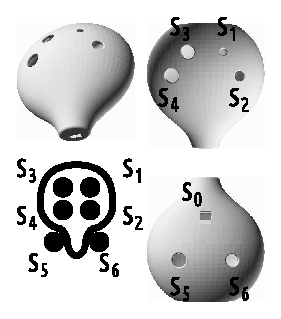
\includegraphics[width=0.750\columnwidth]{ocarina-view.eps}
\caption{View of six-hole ocarina. }
\label{fig:ocarinaview}
\end{figure}
The fingering chart used in this ocarina model is shown in the Table \ref{table:chart} and it is based in the 
4 holes fingering style proposed by John Taylor \citep[pp. 79, 146]{metropolitan1985american} \citep[pp. 30]{1999air}. 
This table indicates the configuration of open or close holes
to produce the tones from $C$ until $D$ (a higher octave), where a value $S_i=1$ represents an 
open hole and the value $S_i=0$ a closed hole.
\begin{table}[h!]
\center
\begin{tabular}{l|c|c|c|c|c|c}
Note & $S_1$ & $S_2$ & $S_3$ & $S_4$ & $S_5$ & $S_6$ \\ \hline
\hline 
$C$  & 0 & 0 & 0 & 0 & 0 & 0 \\
$C\#$& 0 & 0 & 0 & 0 & 0 & 1 \\
$D$  & 1 & 0 & 0 & 0 & 0 & 0 \\
$D\#$& 1 & 0 & 0 & 0 & 0 & 1 \\
$E$  & 0 & 1 & 0 & 0 & 0 & 0 \\
$F$  & 1 & 1 & 0 & 0 & 0 & 0 \\
$F\#$& 0 & 0 & 1 & 0 & 0 & 0 \\
$G$  & 1 & 0 & 1 & 0 & 0 & 0 \\
$G\#$& 0 & 1 & 1 & 0 & 0 & 0 \\
$A$  & 1 & 1 & 1 & 0 & 0 & 0 \\
$A\#$& 1 & 0 & 1 & 1 & 0 & 0 \\
$B$  & 0 & 1 & 1 & 1 & 0 & 0 \\
$C$& 1 & 1 & 1 & 1 & 0 & 0 \\
$C\#$& 0 & 1 & 1 & 1 & 1 & 0 \\
$D$& 1 & 1 & 1 & 1 & 1 & 0 \\
\hline
\end{tabular}
\vspace{5pt}
\caption{Fingering chart}
\label{table:chart}
\end{table}

%%%%%%%%%%%%%%%%%%%%%%%%%%%%%%%%%%%%%%%%%%%%%%%%%%%%%%%%%%%%%%%%%%%%%%%%%%%%%%%%
%%%%%%%%%%%%%%%%%%%%%%%%%%%%%%%%%%%%%%%%%%%%%%%%%%%%%%%%%%%%%%%%%%%%%%%%%%%%%%%%
\section{Math and music}
In this paper we analyze a tuning method with 12 tone in an equal temperament scale; so that, the frequency interval
between any pair of adjacent notes has the same ratio $\rho = {\sqrt[12]{2}}$.
The Table \ref{tab:notes} shows how are distributed the musical notes from tone $C$ until $D$ (a higher octave),
where $f_0$ represents the frequency of $C$ note and the next notes
follow a geometric progression $\hat{f}_{i}={\rho}^i f_{0}$ with $i$ representing the separation degree with the $C$ note. 

\begin{table}[h]
\center
{\renewcommand{\arraystretch}{1.2}
\begin{tabular}{|c|c|c|c|c|}
\hline
$\hat{f}_{0}$ & $\hat{f}_{1}$    & $\hat{f}_{2}$    & $\hat{f}_{3}$    & $\hat{f}_{4}$    \\ \hline
$C$           & $C\#$            & $D$              & $D\#$            & $E$              \\ \hline
$f_{0}$       & ${\rho}^1 f_{0}$ & ${\rho}^2 f_{0}$ & ${\rho}^3 f_{0}$ & ${\rho}^4 f_{0}$ \\ \hline
\hline
$\hat{f}_{5}$    & $\hat{f}_{6}$    & $\hat{f}_{7}$    & $\hat{f}_{8}$    & $\hat{f}_{9}$    \\ \hline
$F$              & $F\#$            & $G$              & $G\#$            & $A$              \\ \hline
${\rho}^5 f_{0}$ & ${\rho}^6 f_{0}$ & ${\rho}^7 f_{0}$ & ${\rho}^8 f_{0}$ & ${\rho}^9 f_{0}$ \\ \hline
\hline 
$\hat{f}_{10}$      & $\hat{f}_{11}$      & $\hat{f}_{12}$      & $\hat{f}_{13}$      & $\hat{f}_{14}$      \\ \hline
$A\#$               & $B$                 & $C$                 & $C\#$               & $D$                 \\ \hline
${\rho}^{10} f_{0}$ & ${\rho}^{11} f_{0}$ & ${\rho}^{12} f_{0}$ & ${\rho}^{13} f_{0}$ & ${\rho}^{14} f_{0}$ \\ \hline
\end{tabular}
}
\vspace{5pt}
\caption{Musical notes}
\label{tab:notes}
\end{table}


\section{Math and ocarina}

\subsection{Analyzing a whistle}
We can think of an ocarina as a whistle with tone-holes in its resonant cavity,
so that when we open and close some of these holes, we can modify the pitch of generated sound.
Thus, to understand the math of an ocarina first we should to know the science behind the whistles  
or more formally a Helmholtz resonant cavity \citep{corning2011resonance} (see Fig. \ref{fig:resonador}) excited by a jet-edge-resonator system (see Fig. \ref{football-referee-whistle}) \citep[pp. 3]{gibiat2013acoustic} \citep[pp. 138]{nyborg1953characteristics}. 
In this sense the Eq. (\ref{eq:Apito}) 
\begin{equation} 
\label{eq:Apito}
 f_0 = \frac{c}{2 \pi} \sqrt{\frac{A_{0}}{l_{0}V} }  
\end{equation}
shows the way of to calculate the frequency $f_0$ of a theoretic\footnote{In  a sphere-like resonant cavity, the open area of the neck should be much less than the total surface area of the resonant cavity.} whistle \citep[pp. 3]{gibiat2013acoustic} \citep[pp. 5]{kobayashi20093d} \citep[pp. 265]{okadanumerical}
in relation with the constants $\pi$  and $c$ (the velocity of sound), and 
the variables: $V$ the volume of its resonant cavity,
$A_0$ its cross-section neck area and $l_0$ the neck effective length in the resonator.


\begin{figure}[ht!]
\centering
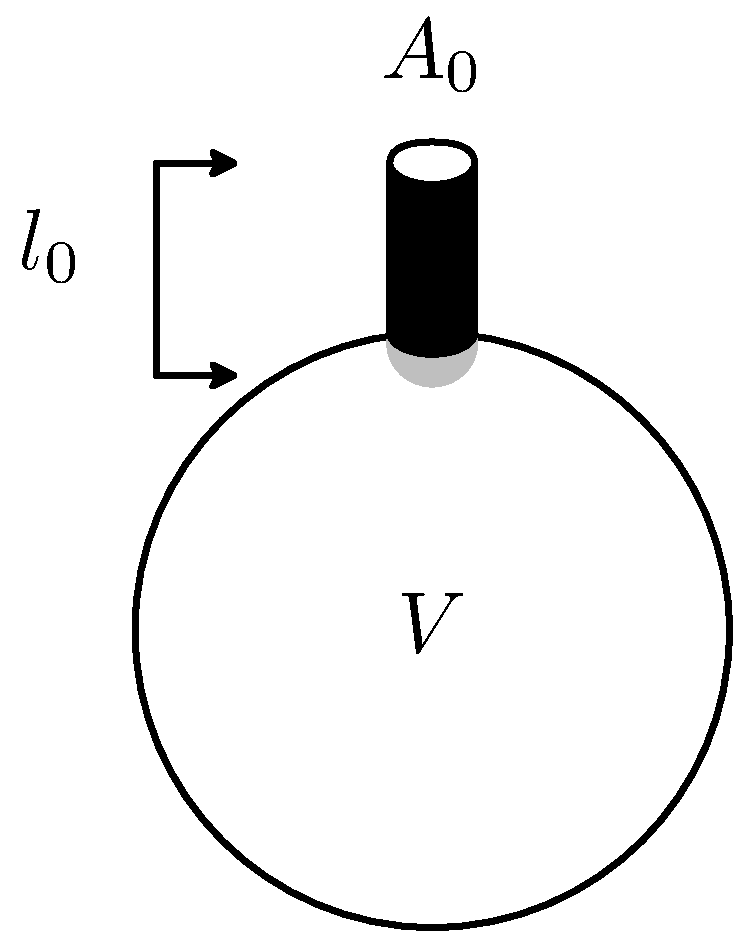
\includegraphics[width=0.350\columnwidth]{resonador.eps}
\caption{whistle. }
\label{fig:resonador}
\end{figure}

\begin{figure}[ht!]
\centering
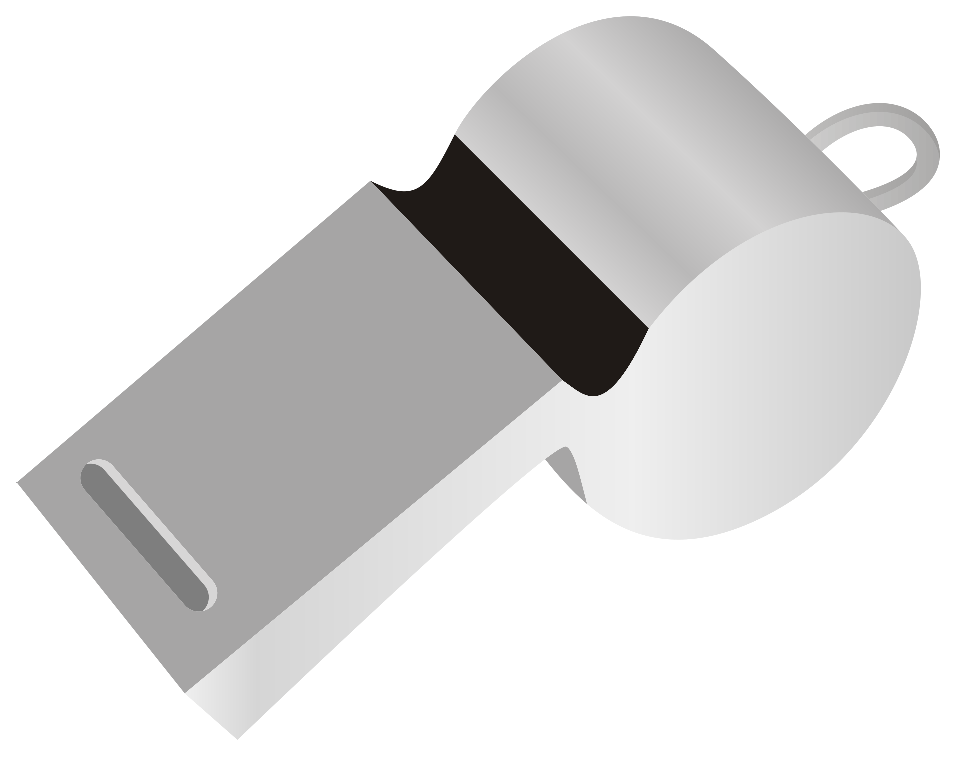
\includegraphics[width=0.250\columnwidth]{football-referee-whistle.eps}
\caption{whistle. }
\label{football-referee-whistle}
\end{figure}

\subsection{Analyzing an ocarina}
\label{subsec:analyzing}
The fundamental resonant frequency $f$ of an ocarina, 
that have at least one circular tone-hole %pitch hole 
in addition to the sound hole (see Fig. \ref{fig:ocarina-teorica}),
can be represented like a function of the total tone-holes area $A$.


\begin{figure}[ht!]
\centering
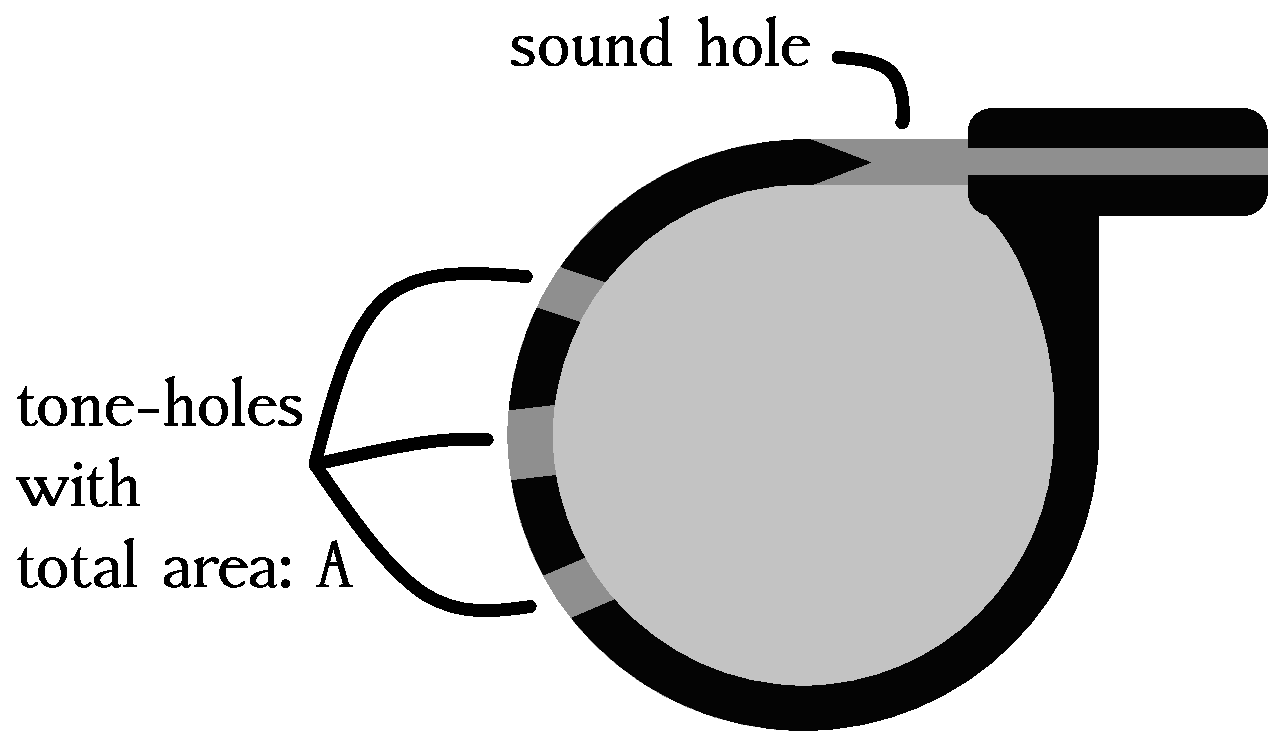
\includegraphics[width=0.750\columnwidth]{ocarina-teorica.eps}
\caption{Theoretic ocarina}
\label{fig:ocarina-teorica}
\end{figure}

In the article ``La Ocarina de Zanahoria a Carrot Ocarina'' \citep{mp2010ocarina}
were analyzed data about of the increment of resonant frequency $f$ in relation to the augment of area $A$,
showing that in that case study the relationships between the variables can be approximated with a line 
\begin{equation}
f=c_1+ c_2~A.
\end{equation}
where $c_1=595.859069$, $c_2=4.324273$ and a mean square error $MSE=8051.1$.
The Fig. \ref{fig:models} shows this linear curve in relation to the collected data.


\begin{figure}[ht!]
\centering
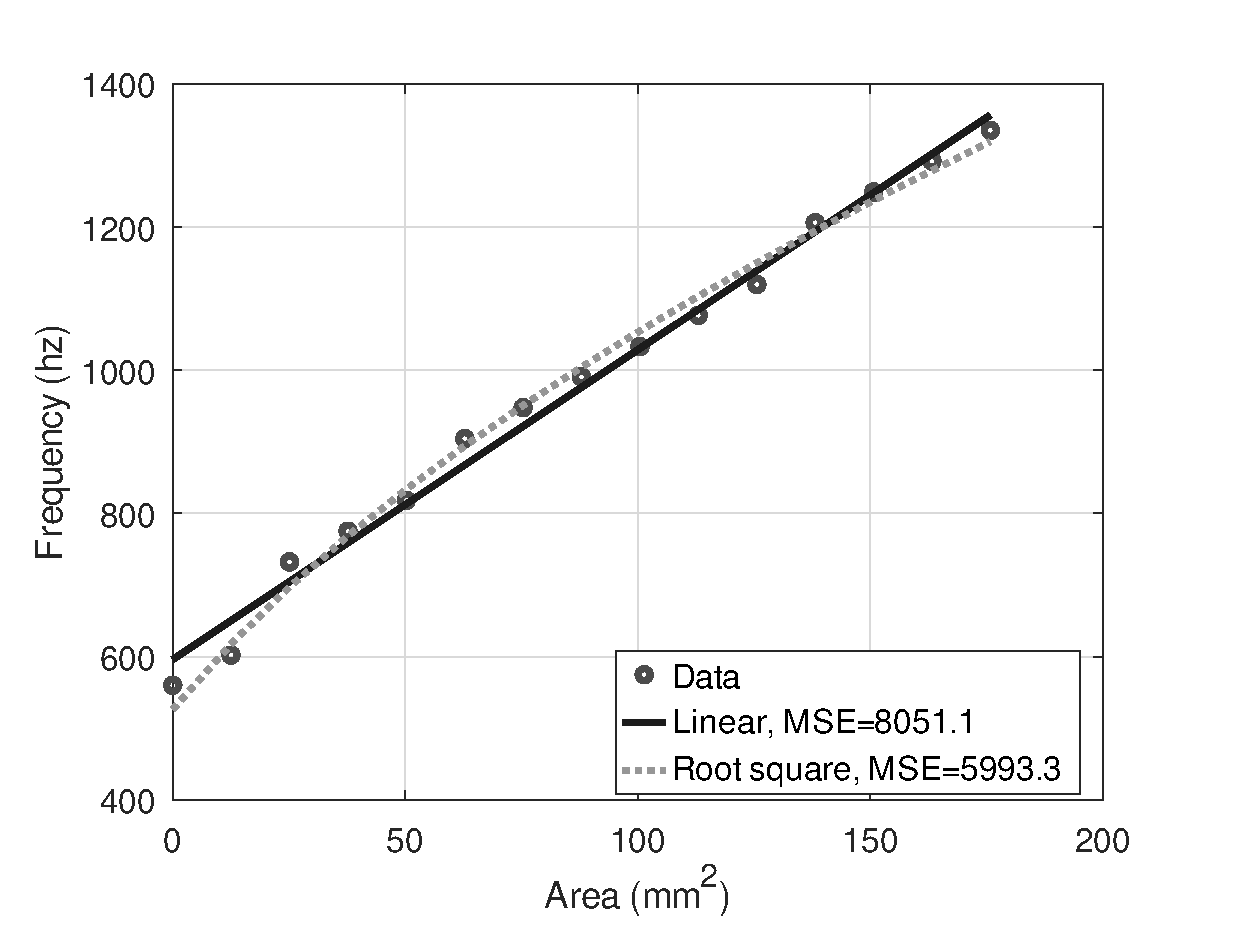
\includegraphics[width=0.850\columnwidth]{compara.eps}
\caption{Comparing models. }
\label{fig:models}
\end{figure}

By other side, 
if we follow the equation proposed by Bart Hopkin in its book ``Air Columns and Toneholes'' 
\citep[pp. 44]{cabreraestudio} \citep[pp. 16]{1999air} and we assume that all the neck effective lengths in the tone-holes are equals,
we can fit the data of Fig. \ref{fig:models} with a square root function
\begin{equation}
f=d_1\sqrt{d_2+A},
\end{equation}
where $d_1=91.215856$, $d_2=33.262474$ and a mean square error $MSE=5993.3$.
We must highlight that in this model $d_2$ represents the area of the sound hole. 

This last model fit better the data, 
also the equation proposed by Hopkin keep coherence with the Helmholtz resonator equation (seen in Eq. (\ref{eq:Apito})).
In the next section we use the model proposed by Hopkin to obtain an optimal tuning in 
John Taylor style six-hole ocarina.


%%%%%%%%%%%%%%%%%%%%%%%%%%%%%%%%%%%%%%%%%%%%%%%%%%%%%%%%%%%%%%%%%%%%%%%%%%%%%%%%
%%%%%%%%%%%%%%%%%%%%%%%%%%%%%%%%%%%%%%%%%%%%%%%%%%%%%%%%%%%%%%%%%%%%%%%%%%%%%%%%
\subsection{Resonance frequency in ocarinas}
\label{subsec:Resonance}
For what is explained in the Sec. \ref{subsec:analyzing}, here 
we use the equation \ref{EcA}, proposed by Bart Hopkin \citep[pp. 44]{cabreraestudio} \citep[pp. 16]{1999air},
\begin{equation} \label{EcA}
 f = \frac{c}{2 \pi} \sqrt{\frac{\frac{A_{0}S_{0}}{l_{0}}+\frac{A_{1}S_{1}}{l_{1}}+\frac{A_{2}S_{2}}{l_{2}}+ . . .}{V} }   
\end{equation}
as a good approximation to estimate the fundamental frequency $f$ 
of globular resonators that have at least one circular pitch hole in addition to the sound hole (a.k.a. an ocarina). 
in which $A_i$ and $l_i$ are the area and the effective length of the $S_i$ tone-hole, 
so that the variable $S_i$ has only two values $\{0,1\}$ according to the Table \ref{table:chart}; 
additionally, $S_0=1$ and represents the sound hole, being $A_0$ and $l_0$ their corresponding variables. 



\subsubsection{Reordering the resonance equation}
We can rearrange the Eq. (\ref{EcA}) defining the variable $h_{i}\propto \frac{A_{i}}{l_{i}}$ 
and the constant $k$, so that
\begin{equation} \label{EcC}
k \equiv \frac{c}{2 {\pi}\sqrt{V}},\qquad  h_{i} \equiv  \frac{A_{i}}{l_{i}}.
\end{equation}
This variable change imply that the Eq. (\ref{EcA}) can be rewritten as
\begin{equation} \label{EcD}
f = k \sqrt{h_0 +\sum_{i=1}^{6}{S_i h_i}},
\end{equation}
It is important to remember that following the Eqs. (\ref{eq:Apito}) and (\ref{EcD}),
when all the tone-holes are closed we obtain that 
\begin{equation} \label{EcDa}
f_0 = k \sqrt{h_0}. %%f(\mathbf{0}) \equiv 
\end{equation}

\subsubsection{Generated frequencies in a six-hole ocarina}

If our intention is to generate by approximation all the 14 frequencies in a six-hole ocarina
similar to seen in Table \ref{tab:notes}, then we 
use the Eq. (\ref{EcD}) to approximate the (note) frequency $f_j(\mathbf{h})$ of the $j$-th row in the Table \ref{table:chart},
\begin{equation} \label{EcDbh}
f_j(\mathbf{h}) = k \sqrt{h_0 +\sum_{i=1}^{6}{S^{j}_{i} h_i}},
\end{equation}
\begin{equation} \label{EcDbvech}
\mathbf{f}(\mathbf{h})=\left[f_1(\mathbf{h}), f_2(\mathbf{h}), ..., f_{14}(\mathbf{h})\right]^{T},
\end{equation}
where the unknown variable $\mathbf{h}=[h_{1},$ $~h_{2},$ $~h_{3},$ $~h_{4},$ $~h_{5},$ $~h_{6}]^T$
and 
the constant $S_{i}^{j}$ is the element of the row $j$ and column $i$ in the matrix $\mathbf{S}$,
\begin{equation}
 \mathbf{S}=
\begin{bmatrix}
0 & 0 & 0 & 0 & 0 & 1 \\
1 & 0 & 0 & 0 & 0 & 0 \\
1 & 0 & 0 & 0 & 0 & 1 \\
0 & 1 & 0 & 0 & 0 & 0 \\ 
1 & 1 & 0 & 0 & 0 & 0 \\ 
0 & 0 & 1 & 0 & 0 & 0 \\
1 & 0 & 1 & 0 & 0 & 0 \\ 
0 & 1 & 1 & 0 & 0 & 0 \\ 
1 & 1 & 1 & 0 & 0 & 0 \\ 
1 & 0 & 1 & 1 & 0 & 0 \\ 
0 & 1 & 1 & 1 & 0 & 0 \\ 
1 & 1 & 1 & 1 & 0 & 0 \\
0 & 1 & 1 & 1 & 1 & 0 \\
1 & 1 & 1 & 1 & 1 & 0 
\end{bmatrix}.
\end{equation}


%%%%%%%%%%%%%%%%%%%%%%%%%%%%%%%%%%%%%%%%%%%%%%%%%%%%%%%%%%%%%%%%%%%%%%%%%%%%%%%%
%%%%%%%%%%%%%%%%%%%%%%%%%%%%%%%%%%%%%%%%%%%%%%%%%%%%%%%%%%%%%%%%%%%%%%%%%%%%%%%%

\section{Problem Statement}



\subsection{Minimization rule and optimal value}
Known and calculated the desired ($\hat{f}_j$) and generated ($f_j(\mathbf{h})$) frequencies 
seen in the Table \ref{tab:notes}  and Eq. (\ref{EcDbh}), respectively.
We propose the next minimization rule
\begin{equation}
\label{eq:minimization}
\begin{matrix}
e^2(\mathbf{h}) & = & \sum\limmits_{j=1}^{14}\left(\frac{f_{j}(\mathbf{h})-\hat{f}_{j}}{\hat{f}_{j}}\right)^2\\
%~ & = & \sum\limmits_{j=1}^{14}\left(1-\frac{f_{j}(\mathbf{h})}{\hat{f}_{j}}\right)^2 \\
~ & = & \sum\limmits_{j=1}^{14}\left(\frac{1}{\rho^j}\sqrt{1+\sum\limmits_{i=1}^{6} \frac{S_{i}^{j} h_i}{h_0}}-1\right)^2.
\end{matrix}
%|| \mathbf{\hat{z}} - \mathbf{z}(\mathbf{h}) ||^2,
\end{equation}
If we define
\begin{equation}\label{eq:varchange}
\mathbf{\hat{h}}=\mathbf{h}/h_0,
\end{equation}
then $e^2(\mathbf{h})$ can be rewritten as
\begin{equation}
e^2(\mathbf{h}) \equiv \hat{e}^2(\mathbf{\hat{h}}) = \left\|\mathbf{g}(\mathbf{\hat{h}})-\mathbf{q}\right\|^2
\end{equation}
where
\begin{equation}
\mathbf{q}=[1,~1,~1,~...,~1]^T,
\end{equation}
\begin{equation}
\mathbf{g}=[g_1(\mathbf{\hat{h}}),~g_2(\mathbf{\hat{h}}),~g_3(\mathbf{\hat{h}}),~...,~g_{14}(\mathbf{\hat{h}})]^T,
\end{equation}
\begin{equation}
g_j (\mathbf{\hat{h}})=\frac{1}{\rho^j}\sqrt{1+\sum\limmits_{i=1}^{6} S_{i}^{j} \hat{h}_i}.
\end{equation}

The minimization problem of Eq. (\ref{eq:minimization}) can be fitted as a case of multiple nonlinear regression 
that can be solved using regularization 
\citep[pp. 129]{pujaicoriverafernando2020}. 
Thus, following this method, we obtain that the vector $\mathbf{\hat{h}}^{*}$, 
\begin{equation}
\mathbf{\hat{h}}^{*}= \underset{\mathbf{\hat{h}}}{\operatorname {arg\,min}}~\hat{e}^2(\mathbf{\hat{h}})
\end{equation}
can be calculated following iteratively the Eq. (\ref{eq:iterativa:1}) 
\small
\begin{equation}\label{eq:iterativa:1}
\begin{array}{l}
\mathbf{\hat{h}}_{l} = \mathbf{\hat{h}}_{l-1}+\\ 
\left\{\mathbf{A}(\mathbf{\hat{h}}_{l-1})^{T} \mathbf{A}(\mathbf{\hat{h}}_{l-1})+\alpha \mathbf{I}\right\}^{-1}
\mathbf{A}(\mathbf{\hat{h}}_{l-1})^{T} \left\{\mathbf{q}-\mathbf{g}(\mathbf{\hat{h}_{l-1}})\right\},
\end{array}
\end{equation}
\normalsize
until $\mathbf{\hat{h}}_{l} \approx \mathbf{\hat{h}}_{l-1}$,
where we declare that $\mathbf{\hat{h}}^{*} \equiv \mathbf{\hat{h}}_{l}$. 

The variables in the Eq. (\ref{eq:iterativa:1}) are the regularization factor $0 \leq \alpha \leq 1.0$ 
(chosen heuristically  by the user), the identity matrix $\mathbf{I}$ and

\begin{equation}
\mathbf{A}(\mathbf{\hat{h}})=
\left[
\begin{matrix}
\DERPAR{g}{h}{1}{1} & \DERPAR{g}{h}{1}{2} & \hdots & \DERPAR{g}{h}{1}{6} \\ 
\DERPAR{g}{h}{2}{1} & \DERPAR{g}{h}{2}{2} & \hdots & \DERPAR{g}{h}{2}{6} \\
\vdots & \vdots & \ddots & \vdots \\ 
\DERPAR{g}{h}{14}{1} & \DERPAR{g}{h}{14}{2} & \hdots & \DERPAR{g}{h}{14}{6} \\
\end{matrix}
\right],
\end{equation}
\begin{equation}
\DERPAR{g}{h}{j}{l}=
\frac{1}{2 \rho^j}\frac{S_{l}^{j}}{\sqrt{1+\sum\limmits_{i=1}^{6} S_{i}^{j} \hat{h}_i}}.
\end{equation}

Thus, following the Eqs. (\ref{eq:varchange}), (\ref{EcDbh}) and (\ref{EcDa}); we obtain the optimum value,
\begin{equation} \label{eq:optimalh}
\mathbf{h}^* = \mathbf{\hat{h}^*}~h_0,
\end{equation}
so that
\begin{equation} \label{EcDbhath}
f_j(\mathbf{\hat{h}^*}~h_0) = f_0 \sqrt{1 +\sum_{i=1}^{6}{S^{j}_{i} \hat{h}^*_i}},
\end{equation}
and consequently (using the Eq. (\ref{EcDbvech}))
\begin{equation} \label{EcDbhathvec}
\mathbf{f}(\mathbf{\hat{h}^*}~h_0)= f_0 \sqrt{1 +\mathbf{S} \mathbf{\hat{h}^*}}.
\end{equation}

\subsection{Iterative calculation}

Using iteratively the Eq. (\ref{eq:iterativa:1}) from $\mathbf{\hat{h}}_0$,
\begin{equation}\label{eq:iterativa:h:0}
\mathbf{\hat{h}}_0=\left[0.25,~0.25,~0.75,~1.0,~1.0,~0.125\right]^{T}
\end{equation}
until $||\mathbf{\hat{h}}_{l}-\mathbf{\hat{h}}_{l-1}||\leq 0.0001$,
we obtain 
\begin{equation}\label{eq:iterativa:h:7}
\mathbf{\hat{h}}_7 = \left[
\begin{matrix}
0.26344\\
0.56628\\
0.98485\\
1.02421\\
1.04440\\ 
0.13352
\end{matrix}
\right],
\end{equation}
with an error $||\mathbf{\hat{h}}_{7}-\mathbf{\hat{h}}_{6}||\equiv 0.000087817$ 
and $e^2(\mathbf{\hat{h}}_{7} h_0)\equiv \hat{e}^2(\mathbf{\hat{h}}_{7} )\equiv 0.0014474$, 
so that $\mathbf{\hat{h}^*} \equiv \mathbf{\hat{h}}_7 $.

\begin{figure}[ht!]
\centering
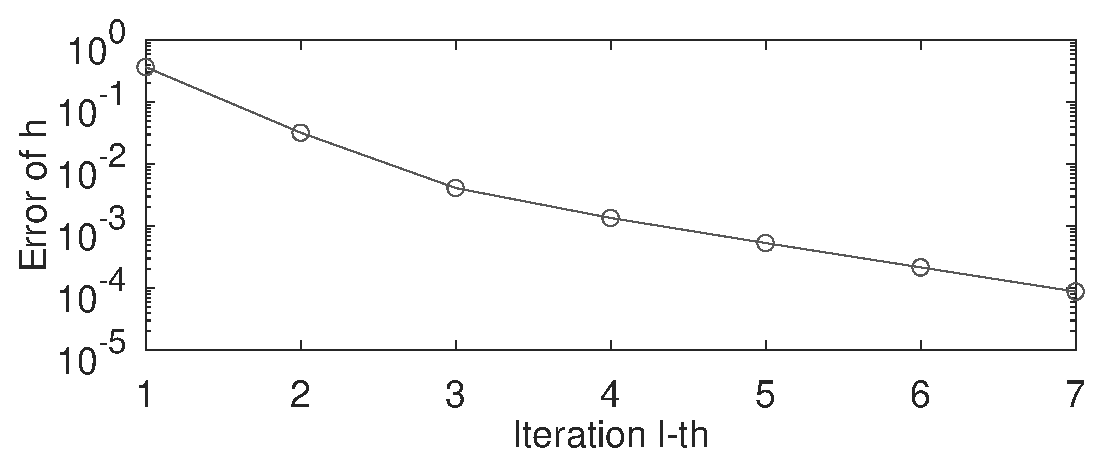
\includegraphics[width=0.950\columnwidth]{errorh.eps}
\caption{Error $||\mathbf{\hat{h}}_{l}-\mathbf{\hat{h}}_{l-1}||$ in consecutive iterations of $\mathbf{\hat{h}}_{l}$.}
\label{fig:errorh}
\end{figure}

Fig. \ref{fig:errorh} shows the error  $||\mathbf{\hat{h}}_{l}-\mathbf{\hat{h}}_{l-1}||$ in consecutive iterations of $\mathbf{\hat{h}}_{l}$,
similarly the Fig. \ref{fig:error} shows the error  $\hat{e}^2(\mathbf{\hat{h}}_{l} )$.


\begin{figure}[ht!]
\centering
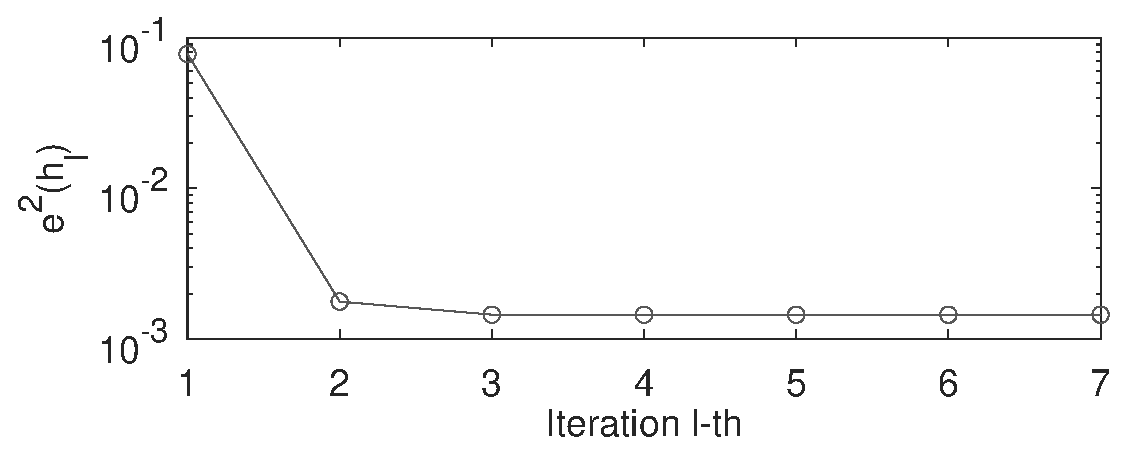
\includegraphics[width=0.950\columnwidth]{error.eps}
\caption{Error $\hat{e}^2(\mathbf{\hat{h}}_{l})$ in consecutive iterations of $\mathbf{\hat{h}}_{l}$.}
\label{fig:error}
\end{figure}

%%%%%%%%%%%%%%%%%%%%%%%%%%%%%%%%%%%%%%%%%%%%%%%%%%%%%%%%%%%%%%%%%%%%%%%%%%%%%%%%
%%%%%%%%%%%%%%%%%%%%%%%%%%%%%%%%%%%%%%%%%%%%%%%%%%%%%%%%%%%%%%%%%%%%%%%%%%%%%%%%
\section{Results}

\begin{mydef}[$E_1$ - relative tuning error ]
\label{def:max:E1}
The first type of error used in this work is 
\begin{equation}
E_1=100~\frac{f_b-f_a}{f_a}~\%,
\end{equation} 
that measures the difference error of $f_b$ in relation to the target frequency ($f_a$),
this error also can be called as relative tuning error.


To obtain the biggest accepted relative tuning error,
it is necessary to know the fact that between any two consecutive notes, with frequencies
$f_a$ and $\rho f_a$, exist a proportion of $\rho\approx 1.059463$ (a semitone), this mean
that the next consecutive note is ever a $+5.9463\%$ that the last note. Thus, 
if we set as maximum error the midway position in geometric proportion between notes, them 
the biggest accepted positive relative tuning error 
to avoid a tone recognition mistake, it is equal to $+2.9302\% \equiv 100 (\sqrt{\rho}f_a-f_a)/f_a~\%$.
By other side 
the biggest accepted negative relative tuning error 
to avoid a tone recognition mistake, it is equal to $-2.8468\% \equiv 100 (f_a/\sqrt{\rho}-f_a)/f_a~\%$.

\end{mydef}

\begin{mydef}[$E_2$ - semitone error]
\label{def:max:E2}
The logarithmic difference error between two frequencies $f_a$ (target) and $f_b$ in relation to a semitone ($\rho$) is
defined as
\begin{equation}
E_2=100~\frac{ln(f_b)-ln(f_a)}{ln(\rho)}~\%, 
\end{equation}
called here as semitone error.


To obtain the biggest accepted semitone error,
we use a similar criterion as seen in the Def. \ref{def:max:E1},
so that 
if we set the maximum error as the midway position in geometric proportion between notes (ex: $C$ and $C\#$), them 
the biggest accepted positive semitone error 
to avoid a tone recognition mistake, it is equal to $+50\% \equiv 100~\frac{ln(\sqrt{\rho} f_a)-ln(f_a)}{ln(\rho)}~\%  $.
By other side 
the biggest accepted negative semitone error 
to avoid a tone recognition mistake, it is equal to $-50\% \equiv 100~\frac{ln( f_a/\sqrt{\rho})-ln(f_a)}{ln(\rho)}~\%  $.
\end{mydef}


\subsection{Analyzing the optimal $\mathbf{h^*}$}
In the Eqs. (\ref{eq:optimalh}) and (\ref{eq:iterativa:h:7}) 
was calculated $\mathbf{h^*}=[h_1^*,$ $h_2^*,$ $...,$ $h_6^*]^{T}$, 
the optimal vector that minimize the function $e^2(\mathbf{h})$. 
The Table \ref{table:h} shows each element of this vector in relation to $h_0$, 
being that $ h_{i}^*/h_{0} \equiv  \left( \frac{l_0}{A_0}\right) \left( \frac{A_{i}}{l_{i}}    \right)$.
\begin{table}[h]
\center
\resizebox{\columnwidth}{!}{%
\begin{tabular}{|c|c|c|c|c|c|}
\hline                           
$h_1^*/h_0$ & $h_2^*/h_0$ & $h_3^*/h_0$ & $h_4^*/h_0$ & $h_5^*/h_0$ & $h_6^*/h_0$ \\ \hline
\hline                           
 26.3\% & 56.6\% & 98.5\% &102.4\% &104.4\% & 13.4\%  \\ \hline 
\end{tabular}}
%\vspace{5pt}
\caption{Percentage ratio between $h_{i}^*$ and $h_{0}$.}
\label{table:h}
\end{table}

In this table we observe that if 
we consider $l_{i}$ a constant throughout the ocarina 
then $h_{i}^*/h_{0} \propto A_{i}$ and 
the percentages presented in the Table \ref{table:h} describe the proportion ratio between areas $A_i$.
So that below this condition 
the optimal area $A_{2}$ is about twice $A_{1}$, 
the optimal area $A_{3}$ is about $3.73 A_{1}$   
and so on.




\subsection{Analyzing the optimal frequencies}

The Tabla \ref{table:res} shows a comparison between the desired 
and optimal generated frequencies for each note in a six-hole ocarina.
\begin{table}[h]
\center
\resizebox{\columnwidth}{!}{%
\begin{tabular}{|l||c|c||r|r|}
\hline 
Note & Desired (hz)& Optimal (hz) & $E_1$ & $E_2$ \\ \hline
\hline 
    $C$ & 1.0000 $f_0$ & 1.0000 $f_0$ &  0.000 \% &   0.000 \% \\ \hline 
  $C\#$ & 1.0595 $f_0$ & 1.0647 $f_0$ &  0.491 \% &   8.483 \% \\ \hline 
    $D$ & 1.1225 $f_0$ & 1.1240 $f_0$ &  0.140 \% &   2.414 \% \\ \hline 
  $D\#$ & 1.1892 $f_0$ & 1.1819 $f_0$ & -0.612 \% & -10.628 \% \\ \hline 
    $E$ & 1.2599 $f_0$ & 1.2515 $f_0$ & -0.667 \% & -11.595 \% \\ \hline 
    $F$ & 1.3348 $f_0$ & 1.3527 $f_0$ &  1.336 \% &  22.974 \% \\ \hline 
  $F\#$ & 1.4142 $f_0$ & 1.4088 $f_0$ & -0.380 \% &  -6.584 \% \\ \hline 
    $G$ & 1.4983 $f_0$ & 1.4994 $f_0$ &  0.075 \% &   1.295 \% \\ \hline 
  $G\#$ & 1.5874 $f_0$ & 1.5972 $f_0$ &  0.619 \% &  10.681 \% \\ \hline 
    $A$ & 1.6818 $f_0$ & 1.6777 $f_0$ & -0.245 \% &  -4.252 \% \\ \hline 
  $A\#$ & 1.7818 $f_0$ & 1.8090 $f_0$ &  1.527 \% &  26.234 \% \\ \hline 
    $B$ & 1.8877 $f_0$ & 1.8909 $f_0$ &  0.165 \% &   2.847 \% \\ \hline 
    $C$ & 2.0000 $f_0$ & 1.9593 $f_0$ & -2.036 \% & -35.613 \% \\ \hline 
  $C\#$ & 2.1189 $f_0$ & 2.1494 $f_0$ &  1.436 \% &  24.685 \% \\ \hline 
    $D$ & 2.2449 $f_0$ & 2.2098 $f_0$ & -1.565 \% & -27.309 \% \\ \hline  
\end{tabular}}
%\vspace{5pt}
\caption{Errors in optimal tuning}
\label{table:res}
\end{table}
The first column shows all notes used in the optimization calculation.
The second column has the desired frequencies $\hat{f}_j$ (equal temperament scale).
The third column has the optimal generated frequencies $f_j$.
The fourth and fifth columns have the errors described in the Definitions \ref{def:max:E1} and \ref{def:max:E2},
respectively.

The worst error $E_1$ is equal to $-2.036\%$ and correspond to the note $C$; 
similarly, this note present the worst error $E_2$ with a detour of $-35.613\%$ of a semitone. 
The next worst error $E_1$ is equal to $-1.565\%$ and correspond to the note $D$,
having an error $E_2$ with a detour of $-27.309\%$ of a semitone.

By the results show in the Table \ref{table:res}, we observe that 
the optimal vector $\mathbf{h^*}$ causes that $e^2(\mathbf{h^*})> 0$
and consequently a perfect equal temperament scale 
it is not possible to be applied in the tuning of a John Taylor style six-hole ocarina,
only it is possible an optimal approximation. 

\subsection{Proposed tuning method}
From the data of the Table \ref{table:res}, 
we can infer an ocarina construction method that fulfill 
an optimal tuning following the minimization rule of the Eq. (\ref{eq:minimization}).
In this sense if we choose of this table a set of notes, 
in which each current note use a new tone-hole in relation to the last tuned note, 
we can obtain a tuning method or sequence to reach an optimal tuning.

With these considerations, the Table \ref{table:example1} shows one tuning method, 
in which is considered a $C$ note equivalent to $523.2511 hz$.
The method consist in follow the table \ref{table:example1} line a line from top at bottom. 
So that we set in our ocarina, with each new created tone-hole, 
the semitone error ($E_2$) shown in the fourth column of the Table \ref{table:example1}.

\begin{table}[h]
\center
\resizebox{\columnwidth}{!}{%
\begin{tabular}{|c||c|c|c|}
\hline                           
Note & Desired (hz) & Optimal (hz) & $E_2$\\ \hline
\hline                           
    $C$ & 523.2511 & 523.2511 &   0.000 \% \\ \hline 
  $C\#$ & 554.3653 & 557.0881 &   8.483 \% \\ \hline 
    $D$ & 587.3295 & 588.1491 &   2.414 \% \\ \hline 
%  $D\#$ & 622.2540 & 618.4455 & -10.628 \% \\ \hline 
    $E$ & 659.2551 & 654.8546 & -11.595 \% \\ \hline 
%    $F$ & 698.4565 & 707.7869 &  22.974 \% \\ \hline 
%  $F\#$ & 739.9888 & 737.1801 &  -6.584 \% \\ \hline 
    $G$ & 783.9909 & 784.5777 &   1.295 \% \\ \hline 
%  $G\#$ & 830.6094 & 835.7495 &  10.681 \% \\ \hline 
%    $A$ & 880.0000 & 877.8411 &  -4.252 \% \\ \hline 
%  $A\#$ & 932.3275 & 946.5632 &  26.234 \% \\ \hline 
    $B$ & 987.7666 & 989.3923 &   2.847 \% \\ \hline 
%    $C$ & 1046.5023 & 1025.1950 & -35.613 \% \\ \hline 
%  $C\#$ & 1108.7305 & 1124.6528 &  24.685 \% \\ \hline 
    $D$ & 1174.6591 & 1156.2749 & -27.309 \% \\ \hline
\end{tabular}}
%\vspace{5pt}
\caption{Proposed tuning method.}
\label{table:example1}
\end{table}


%%%%%%%%%%%%%%%%%%%%%%%%%%%%%%%%%%%%%%%%%%%%%%%%%%%%%%%%%%%%%%%%%%%%%%%%%%%%%%%%
%%%%%%%%%%%%%%%%%%%%%%%%%%%%%%%%%%%%%%%%%%%%%%%%%%%%%%%%%%%%%%%%%%%%%%%%%%%%%%%%
\section{Conclusion}
The results of Table \ref{table:res} shows that it is not possible tuning a John Taylor style six-hole ocarina with a perfect equal temperament scale,
but the minimization rule presented in this work returns a tuning method with an optimal approximation and heterogeneous errors less than $|-35.613\%|$ of a semitone.
Additionally, the Table \ref{table:example1} shows one, of several possibles, construction methods, 
paths or sequences to fulfill an optimal tuning according to the minimization rule defined in the Eq. (\ref{eq:minimization}) and with 
the resonance frequency equation in ocarinas proposed by Bart Hopkin.
This method can be complemented with the information of the relations between areas $A_i$ and effective lengths $l_i$ 
in an optimal tuning shown in the Table \ref{table:h}.


\bibliography{bibliografia}


%\bibitem{JohnTaylorRef}
%[1]https://johntaylorocarina.wordpress.com/2011/05/19/welcome/

\end{document}



